\documentclass{article}
\usepackage{spconf,amsmath,amssymb,amsthm,mathtools,graphicx,hyperref,booktabs}
\usepackage{algorithm}
\usepackage{algpseudocode}

% --------------------------------------------------
% Theorem environments
% --------------------------------------------------
\newtheorem{lemma}{Lemma}
\newtheorem{theorem}{Theorem}
\newtheorem{proposition}{Proposition}
\newtheorem{remark}{Remark}
\usepackage[dvipsnames,table]{xcolor}
% --------------------------------------------------
% Commands
% --------------------------------------------------
\newcommand{\R}{\mathbb{R}}
\newcommand{\Id}{\mathrm{Id}}
\newcommand{\prox}{\operatorname{prox}}
\newcommand{\argmin}{\operatorname*{arg\,min}}
\newcommand{\xb}{\mathbf{x}}
\newcommand{\Ab}{\mathbf{A}}
\newcommand{\Tb}{\mathbf{T}}
\newcommand{\zb}{\mathbf{z}}
\newcommand{\eb}{\mathbf{e}}
\newcommand{\ub}{\mathbf{u}}
% Title.
% ------
\title{Equivariance versus Firm Non-Expansiveness in Incremental Proximal Gradient Methods for Plug-and-Play Denoising}
\name{Sarra Amiri$^{\star}$ \qquad Nelly Pustelnik$^{\star}$ \qquad Jean-Christophe Pesquet$^{\dagger}$}
\address{$^{\star}$~Laboratoire de Physique, ENS de Lyon, CNRS, France \\
         $^{\dagger}$~CVN, CentraleSupélec, Université Paris-Saclay, Inria, France}

\begin{document}
\maketitle

\begin{abstract}
Equivariant Plug-and-Play (PnP) methods symmetrize a learned denoiser by
averaging its action over a group of image transformations, and rely on a
stochastic Monte Carlo approximation for efficiency. We show that when the
denoiser is firmly non-expansive (FNE), this stochastic scheme is not
merely an unbiased estimator: it is closely related to Bertsekas
incremental proximal-subgradient methods, since each randomly conjugated
component is itself the resolvent of a maximal monotone operator. This
gives direct access to Bertsekas convergence guarantees in the special
case where the operator derives from a convex function. We carry out experiments on an SA-UNet denoiser trained with and without an
FNE penalty and with and without equivariance data augmentation. We observe that FNE is the primary driver of both improved equivariance error and reconstruction quality, with augmentation playing a secondary role. Performance nevertheless improves further when the two are combined.
%behind improved equivariance error and reconstruction quality.
\end{abstract}

\begin{keywords}
Plug-and-Play, equivariance, firmly non-expansive denoiser, proximal methods, image restoration, monotone operators
\end{keywords}
\vspace{-0.1cm}

\section{Introduction}
\label{sec:introduction}
\vspace{-0.1cm}

Linear inverse problems in imaging aim to recover an image $\overline{\xb} \in \R^N$
from degraded measurements $\zb = \Ab\overline{\xb} + \eb$, where $\Ab$ models the
acquisition operator (blur, subsampling, \dots) and $\eb$ is the measurement
noise. Since these problems are generally ill-posed, solving them
requires some form of regularization, classically an explicit penalty
term added to the data-fidelity term. \emph{Plug-and-Play} (PnP)
methods offer an alternative: they replace this explicit regularizer
with a pretrained denoiser $\mathbf{D}$, plugged into an iterative
scheme that alternates between a data consistency step and a proximal step imposing regularity to the solution. 

This strategy,
originally heuristic \cite{venkatakrishnan2013plugandplay,zhang2022plugandplay,kamilov2023plug}, has since been given rigorous theoretical
grounding whenever the denoiser satisfies certain stability
properties, in particular firm non-expansiveness (FNE) \cite{Pesquet2021,SantosGarcia2024}, which
guarantees that $\mathbf{D}$ coincides with the resolvent of a maximal
monotone operator \cite{Minty1962} and places PnP squarely within the
classical theory of proximal splitting methods
\cite{CombettesPesquet2011,BauschkeCombettes2017}. Although imposing Lipschitz (or FNE) properties to a neural network is an NP-hard problem \cite{szegedy2013intriguing, Scaman2018Lipschitz} some numerical approaches have been shown to provide reasonable approximations \cite{Neacsu2024a,Neacsu2024b}.

A well-known shortcoming of learned denoisers is that they are not
equivariant to the natural symmetries of images (rotations,
reflections): the same content, shown in a different orientation, is
not necessarily denoised in a consistent way, which can introduce a
directional bias in the reconstruction \cite{chen2023imaging,tachella2026self}. Terris et al.
\cite{Terris2024} address this by symmetrizing the action of the denoiser,
averaging it over a finite group of transformations. They also
introduce a cheaper stochastic variant of this symmetrization, which
they justify as an unbiased Monte Carlo estimator of the averaged
operator. A convergence analysis of the resulting algorithm was provided in \cite{renaud2026equivariant}, under the assumption that the denoiser $\mathbf{D}$ can be expressed as  $\mathbf{D}= \prox_{g}$ for some weakly convex function  $g$. 
This analysis controls the residuals of the iterates and shows that they converge close to critical points. No such analysis has yet been provided within the FNE formalism, which is precisely the focus of this contribution.

Equivariance and the FNE constraint are
usually studied separately in the literature, and it remains debated
which of the two impacts more reconstruction quality.

\noindent \textbf{Contributions.} In this paper, we give a second view of the
stochastic equivariance scheme introduced by Terris et al.: rather
than treating it as a simple stochastic estimator of an averaged
operator, we recast it as an incremental algorithm which coincides with Bertsekas incremental
proximal-subgradient method \cite{Bertsekas2011} under suitable assumptions on the denoiser. We show that, when
the denoiser is FNE, the equivalence is exact: each
randomly drawn component at every iteration is itself the resolvent
of a maximal monotone operator (Lemma~\ref{lem:conjugaison-resolvante}). Moreover, in the special case where this operator derives from a convex
function, it directly inherits from Bertsekas convergence guarantees
(Proposition~\ref{prop:convergence-pas-fixe}). 
We then apply these results in experimental settings, where we train several variants of
the same SA-UNet denoiser \cite{Guo2020SAUNet} (standard, FNE
constrained, trained with equivariance, or combining both) to identify scenarios where equivariance brings a meaningful gain, and
better understand which mechanism, equivariance or the FNE constraint, actually
dominates.

\section{Equivariant Denoising and  Averaging}
\label{sec:equivariant-pnp}

%\noindent \textbf{Reminder: Equivariant PnP}
Plug-and-Play methods build on the idea to replace the proximal operator of an explicit regularizer with a generic denoiser $\mathbf{D}$. Concretely, they rely on the following iterative scheme:
%
\begin{equation}
\label{alg:pnp-base}
(\forall k\in\mathbb{N})\quad
\xb^{[k+1]} =  \mathbf{D}\big(\xb^{[k]} - \tau \Ab^\top (\Ab\xb^{[k]} - \zb)\big).
\end{equation}

%\begin{algorithm}[H]
%\caption{PnP (Plug-and-Play), basic iteration}
%
%\begin{algorithmic}[1]
%\small
%\Require initialization $x_0 \in \R^n$; step size $\alpha>0$; denoiser $D_\sigma$; number of iterations $K$
%\For{$k = 0, 1, \dots, K-1$}
%    \State $z_k \leftarrow x_k - \alpha \nabla f(x_k)$ \Comment{gradient step on the data-fidelity term}
%    \State $x_{k+1} \leftarrow D_\sigma(z_k)$ \Comment{denoising}
%\EndFor
%\State \Return $x_K$
%\end{algorithmic}
%\end{algorithm}

%\subsection{Equivariance and averaging over the group}

%A well-known shortcoming of Algorithm~\ref{alg:pnp-base} is that $D_\sigma$ is generally not equivariant to the natural symmetries of the problem (rotations, reflections), which introduces a directional bias in the reconstruction. 
\noindent \textbf{Equivariance and averaging over the group} -- Terris et al. \cite{Terris2024} propose to
symmetrize the denoiser action by averaging it over a finite group
$\mathcal{G}$ of transformations acting orthogonally on $\R^N$ through
a representation $\mathbf{T}_\ell$ with $\ell\in\mathcal{G}$. In this work, we will focus on the group $\mathcal{G}$ that denotes the dihedral group of order $8$
describing the symmetries of a square (the $4$ rotations
$\{0^\circ,90^\circ,180^\circ, 270^\circ\}$ combined with reflections),
which naturally matches the symmetries of a discrete image on a
square grid. This approach has since been revisited and extended in
later work on equivariant denoising \cite{renaud2026equivariant}. The
equivariant denoising operator is defined as:\vspace{-0.3cm}
\[
  (\forall \xb \in \R^N) \qquad \mathcal{D}_\mathcal{G}(\xb) \;=\; \frac{1}{|\mathcal{G}|}\sum_{\ell \in \mathcal{G}}
  \mathbf{T}_\ell^{-1}\, \mathbf{D}\big(\mathbf{T}_\ell\, \xb\big)
\]\vspace{-0.5cm}

\noindent and the equivariant PnP iteration replaces the denoising step of
Algorithm~\eqref{alg:pnp-base} with $\mathcal{D}_\mathcal{G}$:
$$
 (\forall k=0,1,\dots) \qquad \xb^{[k+1]} = \mathcal{D}_\mathcal{G}\big(\xb^{[k]} - \tau \Ab^\top (\Ab\xb^{[k]} - \zb)\big).
$$
%
\noindent \textbf{Monte Carlo approximation} -- Computing $\mathcal{D}_\mathcal{G}$ requires $|\mathcal{G}|$ calls to
the denoiser at every iteration, which may become expensive. % for groups
%larger than $D_4$ (translation groups, discretized continuous groups,
%\dots). 
Terris et al. \cite{Terris2024} therefore propose a stochastic version, where a
single group element is drawn at each iteration instead of averaging
over all of them:\vspace{-0.6cm}

%
\begin{align}
\label{alg:pnp-mc-terris}
    &\text{For } k=0,1,\dots \nonumber\\
    &\left|
    \begin{aligned}
        &\;\;\text{Select} \;\ell_k \sim \mathcal{U}(\mathcal{G}) \;\text{independently of the previous draws}\\
        &\;\;\xb^{[k+1]} = \mathbf{T}_{\ell_k}^{-1}\, \mathbf{D}\Big(\mathbf{T}_{\ell_k}\big(\xb^{[k]} - \tau \Ab^\top (\Ab\xb^{[k]} - \zb)\big)\Big).
    \end{aligned}
    \right.\raisetag{17pt}
\end{align}\vspace{-0.1cm}

\noindent The authors show experimentally that enforcing equivariance of the denoiser to certain groups of transformations, using this Equivariant-PnP algorithm, strongly improves both the stability of the algorithm and the quality of reconstruction. However, a deeper theoretical investigation is still needed and is provided in the next section.
%\begin{algorithm}[H]
%\caption{Equivariant PnP -- Monte Carlo approximation (Terris et al.)}
%\label{alg:pnp-mc-terris}
%\begin{algorithmic}[1]
%\small
%\Require $x_0 \in \R^n$; step size $\alpha>0$; denoiser $D_\sigma$; group $\mathcal{G}=D_4$ ($|\mathcal{G}|=8$); number of iterations $K$
%\For{$k = 0, 1, \dots, K-1$}
%    \State $z_k \leftarrow x_k - \alpha \nabla f(x_k)$
%    \State Draw $g_k \sim \mathcal{U}(\mathcal{G})$, independently of the past
%    \State $x_{k+1} \leftarrow T_{g_k}^{-1}\, D_\sigma\big(T_{g_k}\, z_k\big)$
%\EndFor
%\State \Return $x_K$
%\end{algorithmic}
%\end{algorithm}


\section{A Bertsekas formulation of the Monte Carlo Equivariant PnP}
\label{sec:bertsekas-reading}

We now give a new interpretation of Algorithm~\eqref{alg:pnp-mc-terris},
which no longer treats it as a simple stochastic estimator of
$\mathcal{D}_\mathcal{G}$, but instead as an instance of Bertsekas
incremental proximal-subgradient methods \cite{Bertsekas2011}. This re-interpretation allows us to benefit from the well-established convergence results in some specific settings.\\\vspace{-0.2cm}

%The starting point of both approaches is the same: at every iteration, a single element $\ell_k$ of the group is drawn at random, independently of the past, uniformly over $\mathcal{G}$.

\noindent \textbf{FNE and orthonormal transforms} --  Suppose that $\mathbf{D}$ is firmly non-expansive, defined on the whole space. By Minty's
theorem \cite{Minty1962}, there then exists a maximal monotone
operator $\mathbf{M}\colon\R^N \rightrightarrows\R^N$ such that
$\mathbf{D} \;=\; \mathrm{J}_{\mathbf{M}} \;:=\; (\Id+\mathbf{M})^{-1}$,
where $\mathrm{J}_{\mathbf{M}}$ denotes the resolvent of $\mathbf{M}$. The following lemma, a
classical result in monotone operator theory (see \cite{CombettesPesquet2011,BauschkeCombettes2017}), shows that this structure is preserved
under orthogonal conjugation:

\begin{lemma}[Invariance of the resolvent under orthogonal conjugation]
\label{lem:conjugaison-resolvante}
Let $\mathbf{M}$ be a maximal monotone operator on $\R^N$, and let $\mathbf{T}_\ell$ be an
orthogonal transformation. Then
\[
  \mathrm{J}_{\widetilde{\mathbf{M}}_\ell} = \mathbf{T}_\ell^{-1} \circ \mathrm{J}_{\mathbf{M}}  \circ \mathbf{T}_\ell \quad \text{where} \quad \widetilde{\mathbf{M}}_\ell := \mathbf{T}_\ell^{-1} \mathbf{M}\, \mathbf{T}_\ell,
\]
and $\widetilde{\mathbf{M}}_\ell$ is also a maximal monotone operator.
\end{lemma}

So for every $\ell \in \mathcal{G}$, the term $\mathbf{T}_\ell^{-1}   \mathbf{D} \mathbf{T}_\ell$ used
in Algorithm~\eqref{alg:pnp-mc-terris} is itself exactly the resolvent
of a maximal monotone operator $\widetilde{\mathbf{M}}_\ell := \mathbf{T}_\ell^{-1} \mathbf{M}\, \mathbf{T}_\ell$. We can
therefore rewrite the algorithm in a form that implies a \textit{randomized resolvent interpretation} involving maximal monotone
operators :
\begin{align}
\label{alg:pnp-mc-terris-J}
    &\text{For } k=0,1,\dots \nonumber\\
    &\left|
    \begin{aligned}
        &\;\;\text{Select} \;\ell_k \sim \mathcal{U}(\mathcal{G}) \;\text{independently of the previous draws}\\
        &\;\; \widetilde{\mathbf{M}}_{\ell_k} := \mathbf{T}_{\ell_k}^{-1} \mathbf{M}\, \mathbf{T}_{\ell_k}\\
        &\;\;\xb^{[k+1]} = \mathrm{J}_{\widetilde{\mathbf{M}}_{\ell_k}} \big(\xb^{[k]} - \tau \Ab^\top (\Ab\xb^{[k]} - \zb)\big).
    \end{aligned}
    \right.\raisetag{17pt}
\end{align}\vspace{-0.1cm}
%
%\begin{algorithm}[H]
%\caption{Equivariant PnP -- operator-based reading (FNE case)}
%\label{alg:pnp-mc-operateur}
%\begin{algorithmic}[1]
%\small
%\Require $x_0 \in \R^n$; step size $\alpha>0$; maximal monotone operator $A$ such that $D_\sigma = J_A$; group $\mathcal{G}=D_4$
%\For{$k = 0, 1, \dots, K-1$}
%    \State $z_k \leftarrow x_k - \alpha \nabla f(x_k)$
%    \State Draw $g_k \sim \mathcal{U}(\mathcal{G})$, independently of the past
%    \State $A^{g_k} \leftarrow T_{g_k}^{-1} A\, T_{g_k}$ \Comment{orthogonal conjugation of $A$, Lemma~\ref{lem:conjugaison-resolvante}}
%    \State $x_{k+1} \leftarrow J_{A^{g_k}}(z_k)$
%\EndFor
%\State \Return $x_K$
%\end{algorithmic}
%\end{algorithm}
%

\noindent This change of viewpoint that consists in replacing \textit{a randomly orthogonal conjugated
resolvent} with the \textit{resolvent of a random operator $\widetilde{\mathbf{M}}_{\ell_k}$} drawn
from a finite family, is exactly what lets us step directly into
Bertsekas framework.%, in the special case where $\mathbf{M}$ derives from a convex function. 
\\\vspace{-0.2cm}

%
\noindent \textbf{Special case: $\mathbf{M}$ subdifferential of a convex function} -- When the maximal monotone operator is a convex subdifferential, we show that the method becomes a
randomized incremental proximal method of Bertsekas \cite{Bertsekas2011}. The case where the denoiser is associated with an explicit regularizer corresponds
to $\mathbf{M} = \tau \partial \phi$, for some proper closed convex function $\phi :
\R^N \to \mathbb{R}$ and $\tau>0$. The resolvent $\mathrm{J}_{\mathbf{M}}$ is then exactly the
proximal operator:
\begin{equation*}
(\forall \xb\in \mathbb{R}^N) \qquad   \mathbf{D}(\xb) = \mathrm{J}_{\tau \partial \phi}(\xb) = \prox_{\tau\phi}(\xb)
\end{equation*}
In that specific case, $\mathbf{D}$ is FNE and it fits exactly the setting of \cite{Bertsekas2011} where
each $\ell \in \mathcal{G}$ corresponds to a component $\phi_\ell := \phi
\circ T_\ell$ (also convex, lower semicontinuous, and proper, since $T_\ell$ is an
isometry), and the incremental iteration alternates a gradient step
on the data-term with a proximal step on the randomly drawn component
$\phi_{\ell_k}$:%, projected onto a constraint set $X \subset \R^n$ (for instance $X=\R^n$ when there is no explicit constraint):
%
\begin{align}
\label{alg:pnp-mc-proximal}
    &\text{For } k=0,1,\dots \nonumber\\
    &\left|
    \begin{aligned}
        &\;\;\text{Select} \;\ell_k \sim \mathcal{U}(\mathcal{G}) \;\text{independently of the previous draws}\\
        &\;\; \phi_{\ell_k} = \phi \circ \mathbf{T}_{\ell_k}\\
        &\;\;\xb^{[k+1]} = \prox_{\tau_k\phi_{\ell_k}} \big(\xb^{[k]} - \tau_k \Ab^\top (\Ab\xb^{[k]} - \zb)\big).
    \end{aligned}
    \right.\raisetag{17pt}
\end{align}

%\begin{algorithm}[H]
%\caption{Equivariant PnP -- proximal reading (case $A=\partial\phi$)}
%\label{alg:pnp-mc-proximal}
%\begin{algorithmic}[1]
%\small
%\Require $x_0 \in X$; step size $\alpha>0$; convex function $\phi$; group $\mathcal{G}=D_4$; constraint set $X \subset \R^n$
%\For{$k = 0, 1, \dots, K-1$}
%    \State $z_k \leftarrow x_k - \alpha \nabla f(x_k)$
%    \State Draw $g_k \sim \mathcal{U}(\mathcal{G})$, independently of the past
%    \State $\phi_{g_k} \leftarrow \phi \circ T_{g_k}$
%    \State $x_{k+1} \leftarrow \prox_{\alpha \phi_{g_k}}(z_k) = \displaystyle\argmin_{x \in X} \Big\{ \phi_{g_k}(x) + \tfrac{1}{2\alpha}\|x-z_k\|^2 \Big\}$
%\EndFor
%\State \Return $x_K$
%\end{algorithmic}
%\end{algorithm}

Building on this framework, we can consider Bertsekas convergence results in terms of function value to derive the following statement, specified to our setting, in the fixed-step-size case.
%\begin{proposition}[Convergence with a fixed step size]
%\label{prop:convergence-pas-fixe}
%For every $\xb\in \mathbb{R}^N$, let $F(\xb) :=\frac{1}{2}\Vert \Ab \xb - \zb \Vert_2^2 + \sum_{\ell=1}^L\phi(\mathbf{T}_\ell \xb)$ with $\zb\in \mathbb{R}^M$, $\Ab\in \mathbb{R}^{M\times N}$, $\phi\colon \mathbb{R}^N \to (-\infty,+\infty]$ a convex, lower-semicontinuous, and proper function, and $(\mathbf{T}_\ell)_{1\leq \ell \leq L}$ a family of orthonormal transforms. Let $(\xb^{[k]})_{k\in \mathbb{N}}$ be the sequence generated by
%Algorithm~\eqref{alg:pnp-mc-proximal} with a constant step size
%$\tau_k \equiv \tau$, and $F^\star := \inf_{\xb\in \mathbb{R}^N} F(\xb)$.
%Then, with probability 1:\vspace{-0.1cm}
%\begin{enumerate}
%  \item[(i)] if $F^\star = -\infty$, then $\inf_{k\ge0} F(\xb^{[k]}) = -\infty$;\vspace{-0.2cm}
%  \item[(ii)] if $F^\star > -\infty$, then 
%$    \inf_{k\ge 0} F(\xb^{[k]}) \;\le\; F^\star + \frac{\tau\,\beta\,|\mathcal{G}|\,c^2}{2}.$
%\end{enumerate}
%\end{proposition}
\begin{proposition}[Fixed-step objective-value bound]
\label{prop:convergence-pas-fixe}
For every $\xb\in \mathbb{R}^N$, let $F(\xb) :=\frac{1}{2}\Vert \Ab \xb - \zb \Vert_2^2 + L^{-1}\sum_{\ell=1}^L\phi(\mathbf{T}_\ell \xb)$ with $\zb\in \mathbb{R}^M$, $\Ab\in \mathbb{R}^{M\times N}$, $\phi\colon \mathbb{R}^N \to \mathbb{R}$ a convex, lower-semicontinuous, and proper function, and $(\mathbf{T}_\ell)_{1\leq \ell \leq L}$ a family of orthonormal transforms.  Let $(\xb^{[k]})_{k\in \mathbb{N}}$ be the sequence generated by
Algorithm~\eqref{alg:pnp-mc-proximal} with a constant step size
$\tau_k \equiv \tau$, and $F^\star := \inf_{\xb\in \mathbb{R}^N} F(\xb)$ and assume that there exists $c\in\mathbb{R}$ such that, with probability 1,  
$
\max\Big\{\big\|\nabla\big(\tfrac{1}{2}\|\Ab \xb^{[k]}-\zb\|_2^2\big)\big\|,\ \|\partial \phi(\mathbf{T}_{\ell_k} \xb^{[k]})\|\Big\} \le c$, for every $\ell_k \in \mathcal{G}$.
Then, with probability 1:\vspace{-0.3cm}
\begin{enumerate}
  \item[(i)] if $F^\star = -\infty$, then $\inf_{k\ge0} F(\xb^{[k]}) = -\infty$;\vspace{-0.3cm}
  \item[(ii)] if $F^\star > -\infty$, then 
$    \inf_{k\ge 0} F(\xb^{[k]}) \;\le\; F^\star + \frac{5\tau\,c^2}{2}.$
\end{enumerate}
%Here $c$ is a uniform bound on the (sub)gradients involved at each iteration: 
%where $\ub_{\ell_k} = \prox_{\tau\phi(\mathbf{T}_{\ell_k} \cdot)}(\xb^{[k]})$.
\end{proposition}

In other words, with a fixed step size, the sequence does not
converge exactly to $F^\star$, but 
the result guarantees that the iterates attain objective values within an \(O(\tau)\) neighborhood of the optimum.
The error bound decreases linearly with $\tau$.%,
%at the cost of slower convergence.
\vspace{-0.3cm}

\section{Experiments}
\label{sec:experiences}
\vspace{-0.2cm}

Our experiments are run with Deep Inverse
project library \cite{Tachella2025} on a standard restoration problem where $\Ab$ denotes a Levin blur kernel and $\eb$ a white Gaussian noise with standard deviation set to $\sigma = 0.03$.  We run Algorithm~\eqref{alg:pnp-mc-terris} with several denoisers that share the same architecture but differ in training, depending on whether the FNE property and/or equivariance are enforced during training. Our main goal is to evaluate the impact of using an FNE denoiser within Algorithm~\eqref{alg:pnp-mc-terris}. Note that Proposition~\ref{prop:convergence-pas-fixe} guarantees error bound decreasing only when in the convex regularization setting, and its extension to the FNE case has not been established; we therefore restrict our analysis to an empirical evaluation.

\noindent \textbf{Choice of denoiser: SA-UNet} -- Throughout our experiments, we use a SA-UNet
(\emph{Spatial Attention U-Net}) \cite{Guo2020SAUNet}, an architecture
originally proposed for retinal vessel segmentation, which we adapt
here to image denoising. SA-UNet follows the classic
encoder--decoder structure of U-Net, with skip connections between
matching levels of the encoder and decoder. %Figure~\ref{fig:sa-unet}
%shows the overall architecture.
%\hspace{+0.25cm}
%\begin{figure}[t]
%    \centering
%    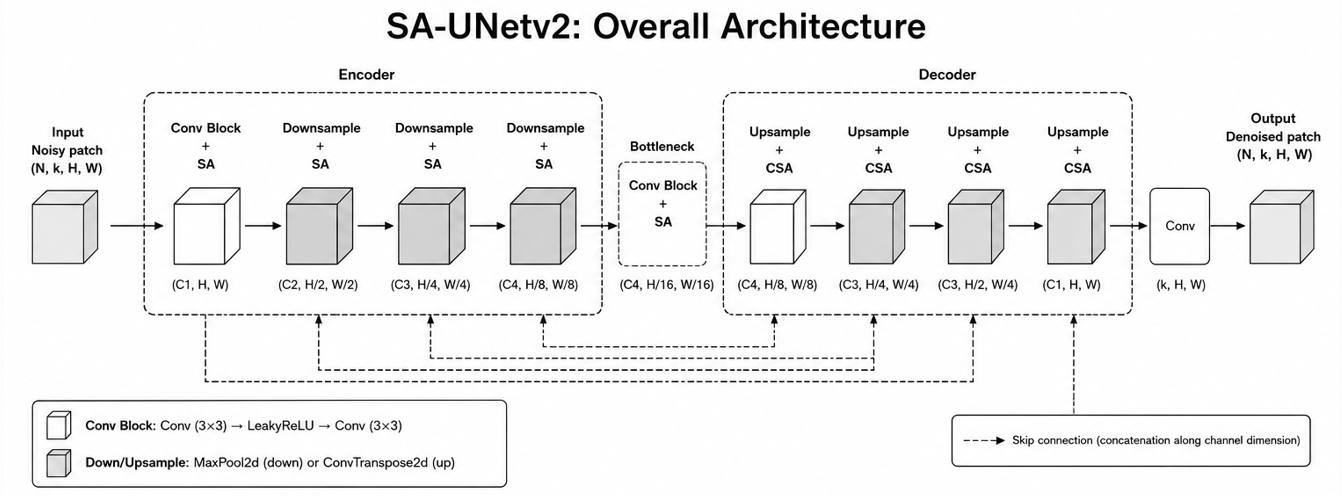
\includegraphics[width=1.15\linewidth]{image.png}
%    \caption{Overview of the SA-UNet architecture.}
%    \label{fig:sa-unet}
%\end{figure}

%\begin{itemize}
%    \item \textbf{Conv Block (ConvGNAct)}: a $3\times3$ convolution
 %   with no bias, followed by a DropBlock (spatially structured
  %  dropout), then GroupNorm and a SiLU activation. Each level
   % applies this block twice (DoubleConvSA).

 %   \item \textbf{Downsampling (DownSA)}: a $2\times2$ max-pooling
 %   layer halves the spatial resolution, followed by a DoubleConvSA
  %  that doubles the number of channels to extract larger-scale
   % features.

    %\item \textbf{Spatial Attention (SA)}: at the bottleneck, we
    %compute the mean and max over the channel axis, concatenate
    %them, then apply a $7\times7$ convolution followed by a sigmoid
    %to produce an attention map with values in $[0,1]$ that
    %reweights features spatially.

 %   \item \textbf{Cross-Scale Spatial Attention (CSA)}: combines the
 %   channel-wise mean of the encoder skip connection and of the
 %   decoder feature map (at matching resolution) through a
 %   $7\times7$ convolution followed by a sigmoid, producing a map
 %   that filters the skip connection before concatenation, reducing
 %   the noise it carries.

 %   \item \textbf{Upsampling (UpSA)}: a $2\times2$ transposed
 %   convolution doubles the resolution, padding corrects odd input
 %   sizes, and the CSA-filtered skip connection is concatenated with
 %   the upsampled feature map before a final DoubleConvSA.
%\end{itemize}

%Fixed-point theory tells us that the FNE constraint is necessary to
%guarantee PnP convergence, while opinions on the actual benefit of
%equivariance seem to be split in the literature. Our goal in this
%section is therefore to provide better insight on this question.
%work out \textbf{under which scenarios
%equivariance brings a meaningful gain, and which mechanism --
%equivariance or the FNE constraint -- actually dominates}. To do
%this, we compare the following algorithms:

%\begin{itemize}
%  \item the base PnP algorithm (Algorithm~\ref{alg:pnp-base}), using
%  either the standard SA-UNet denoiser, its FNE-constrained variant,
%  or its equivariance-trained variant;
 % \item the equivariant PnP algorithm (Algorithms~\ref{alg:pnp-mc-terris}
%  through~\ref{alg:pnp-mc-proximal}), again using, separately, a base
 % denoiser or an FNE denoiser.
%\end{itemize}


\noindent\textbf{Training} -- The denoisers are trained on a subset of ImageNet containing
$50{,}000$ images, split into $45\times45$ patches. Additive
Gaussian noise at level $\sigma=0.03$ is used to generate noisy
observations 
$\mathbf{y} = \overline{\xb} + \mathbf{n}$ where $\mathbf{n} \sim \mathcal{N}(0,\sigma^2 I)$. 
The training follows the protocol proposed by Pesquet et al.
\cite{Pesquet2021}, which adds to the denoising loss a penalty that
encourages the denoiser to be firmly non-expansive. Writing $\mathbf{D}:=\mathbf{D}_\theta$
for the denoiser parameterized by $\theta$ and $\mathbf{Q}_\theta :=
2\mathbf{D}_\theta - \Id$, the loss function is\vspace{-0.2cm}
{\small{\[
  \mathcal{L}(\theta)=\sum_{i=1}^{B}\frac{\big\|\mathbf{D}_\theta(\mathbf{y}_i)-\xb_i\big\|^2}{2BP^2}
  +
  \lambda \max\big(\big\|J_{\mathbf{Q}_\theta}(\tilde{\xb})\big\|_2 - (1-\epsilon), 0\big)^2
\]}}\vspace{-0.4cm}

\noindent \!\!where $B$ is the batch size, $P$ the patch size,
$\lambda>0$ controls the strength of the FNE constraint,
$\epsilon>0$ is a margin parameter, and $\tilde{\xb}$ is the point at
which the spectral norm of the Jacobian $J_{\mathbf{Q}_\theta}$ is evaluated.
This penalty encourages $\mathbf{Q}_\theta$ to be non-expansive and, in turn,
$\mathbf{D}_\theta$ to be firmly non-expansive \cite{Pesquet2021}. We therefore consider four denoiser variants:\vspace{-0.3cm}
\begin{itemize}
\item \textbf{SA-UNet base}: standard training, with $\lambda=0$;\vspace{-0.3cm}
\item \textbf{SA-UNet equiv.}: training with data augmentation
using the transformations of the group $D_4$ with $\lambda=0$;\vspace{-0.3cm}
\item \textbf{SA-UNet FNE}: training with the FNE (i.e, $\lambda>0$);\vspace{-0.3cm}
\item \textbf{SA-UNet FNE + equiv.}: combining the FNE penalty (i.e, $\lambda>0$)
with $D_4$ augmentation.\vspace{-0.3cm}
\end{itemize}
%summarized in
%Table~\ref{tab:variantes-saunet}:
For FNE-based training, $\lambda$ has been selected to minimize the spectral
norm of the Jacobian of $\mathbf{Q}_\theta$.
Optimization is carried out with Adam. Models with the FNE constraint
are obtained by fine-tuning the corresponding denoiser, while the
equivariant models are trained by taking the group $\mathcal{G}$ that denotes the dihedral group of order $8$
describing the symmetries of a square (the $4$ rotations
$\{0^\circ,90^\circ,180^\circ, 270^\circ\}$ combined with reflections).



Table~\ref{tab:perf_denoiser} reports, for the four variants of denoiser and on a test patch of size
$45\times45$ taken from a reference image, the average equivariance
error $E_{\mathrm{eq}}^{\mathrm{moy}}$ (with its standard deviation
$E_{\mathrm{eq}}^{\sigma}$), together with the deviation from the
non-expansiveness constraint $\sigma_{\mathrm{FNE}}$ (the spectral
norm of the Jacobian of $\mathbf{Q}_\theta$, estimated with 50
iterations of the power method, which should ideally be no larger than $1$) and
its absolute and relative residuals. \vspace{-0.2cm}

%\begin{figure*}
%\begin{tabular}{cc}
%     \includegraphics[width = 8cm]{figures_chateau/crit.png}&\includegraphics[width = 8cm]{figures_mante/crit.png}\\  \includegraphics[width = 8cm]{figures_chateau/psnr.png}  & \includegraphics[width = 8cm]{figures_mante/psnr.png}\\
%\end{tabular}
%\end{figure*}



\begin{table}[H]
\centering
\scriptsize
\renewcommand{\arraystretch}{0.95}
\begin{tabular}{lccccc}
\toprule
\textbf{Method}
& $E_{\mathrm{eq}}^{\mathrm{moy}}$
& $E_{\mathrm{eq}}^{\sigma}$
& $\sigma_{\mathrm{FNE}}$
& Abs. res.
& Rel. res. \\
\midrule
SA-UNet base
& 0.015 & 0.006 & 10.080 & 1.377 & 0.022 \\
SA-UNet  Equiv.
& 0.005 & 0.002 & 2.198 & 0.455 & 0.007 \\
SA-UNet  FNE
& 0.003 & 0.001 & 0.994 & 0.310 & 0.005 \\
SA-UNet FNE + Equiv.
& 0.002 & 0.001 & 0.994 & 0.344 & 0.005 \\
\bottomrule
\end{tabular}
\caption{Denoiser performance.
}\vspace{-0.4cm}
\label{tab:perf_denoiser}
\end{table}

\noindent \textbf{Compared PnP variant} -- Using these denoisers, we evaluate six PnP implementations:\\
\hspace*{0.1cm} $\bullet$ \textbf{PnP}: Algorithm~\eqref{alg:pnp-base} with SA-UNet base;\\
\textit{Standard PnP procedure.}\\
\hspace*{0.1cm}$\bullet$ \textbf{PnP-Equiv.}: Algorithm~\eqref{alg:pnp-base} with SA-UNet equiv;\\
\textit{Standard PnP procedure when the training involved equivariant augmentation.}\\
\hspace*{0.1cm}$\bullet$  \textbf{PnP-FNE}: Algorithm~\eqref{alg:pnp-base} with SA-UNet FNE;\\
 \textit{Implementation from \cite{Pesquet2021}.}\\
\hspace*{0.1cm}$\bullet$  \textbf{PnP-FNE-Equiv}: Algo.~\eqref{alg:pnp-base} with SA-UNet FNE + Equiv;\\
\textit{Implementation from \cite{Pesquet2021} when the training involved equivariant augmentation.}\\
$\bullet$  \textbf{Bert-PnP}: Algorithm~\eqref{alg:pnp-mc-terris} with SA-UNet base;\\
\hspace*{0.1cm}  \textit{Implementation provided in \cite{Terris2024}.}\\
\hspace*{0.1cm}$\bullet$   \textbf{Bert-PnP-FNE} (Proposed): Algo.\eqref{alg:pnp-mc-terris} with SA-UNet FNE.\\\vspace{-0.2cm}

%\textbf{PnP} refers to the standard PnP procedure. \textbf{PnP-Eq} refers to the standard PnP procedure when the training involved equivariant augmentation. \textbf{PnP-FNE} refers to the method of \cite{Pesquet2021}. \textbf{PnP-FNE-Eq} refers to the method of \cite{Pesquet2021} when the training involved equivariant augmentation. \textbf{Bert-PnP} refers to the implementation provided in \cite{Terris2024}. \textbf{Bert-PnP-FNE} refers to \cite{Terris2024} when an FNE denoiser is used. In these procedure \textbf{PnP-FNE} is insured to converge in a general setting. %\textcolor{blue}{comment egalement mettre en avant guaraties plus forte pour PnP-FNE (Bert.) alors que resultat uniquement pour fonctions ?}



%This table shows that the FNE constraint appears to be the more decisive mechanism. By choosing the best hyperparameters, we were able to obtain a denoiser that satisfies both properties we look for. One particularly interesting result is that the FNE constraint reduces the average equivariance error more strongly than training with equivariance data augmentation does. Combining both approaches naturally gives the best results, with the FNE~+~Equivariant model performing best overall. That said, we get different results on another image.

%\begin{table}[H]
%\centering
%\scriptsize
%\renewcommand{\arraystretch}{0.95}
%\begin{tabular}{lccccc}
%\textbf{Method}
%& $E_{\mathrm{eq}}^{\mathrm{moy}}$
%& $E_{\mathrm{eq}}^{\sigma}$
%& $\sigma_{\mathrm{FNE}}$
%& Abs. res.
%& Rel. res. \\
%\midrule
%SA-UNet (base)
%& 0.010885 & 0.004172 & 1.138828 & 2.063999 & 0.045643 \\
%Equivariant
%& 0.032661 & 0.012392 & 1.043930 & 2.909145 & 0.064332 \\
%FNE (best)
%& 0.004438 & 0.001702 & 0.991420 & 0.808145 & 0.017871 \\
%FNE (best) 
%& 0.004083 & 0.001573 & 1.017848 & 0.804795 & 0.017797 \\
%+ Equivariant
%\end{tabular}
%\caption{Denoiser performance, random image.}
%\label{tab:perf_denoiser_random}
%\end{table}

%\textbf{The reader is lost. We have the feeling that our
%conclusions are unstable. In addition, we do not know what is this ``random image" and how it makes sense.}
%On this random image, we see that adding the equivariance constraint
%can, in some cases, actually increase the model's equivariance error
%instead of reducing it. This mostly shows that equivariance
%performance can depend on the image being tested, and is therefore
%not necessarily consistent from one image to another.

%That said, one result is clearly confirmed by this experiment: the
%FNE constraint remains the most dominant mechanism. It produces the
%largest reduction in average equivariance error and also keeps
%$\sigma_{\mathrm{FNE}}$ close to 1. Adding the equivariance
%constraint on top of FNE brings a further, though smaller,
%improvement.

%\begin{table}[H]
%\centering
%\scriptsize
%\renewcommand{\arraystretch}{1.5}
%\begin{tabular}{lccccc}
%\toprule
%\textbf{Method}
%& $E_{\mathrm{eq}}^{\mathrm{moy}}$
%& $E_{\mathrm{eq}}^{\sigma}$
%& $\sigma_{\mathrm{FNE}}$
%& Abs. res.
%& Rel. res. \\
%\midrule
%SA-UNet (base)
%& 0.02147 & 0.00824 & 10.25839 & 1.22517 & 0.04661 \\
%Equivariant
%& 0.02010 & 0.00767 & 3.78165  & 0.74320 & 0.02828 \\
%FNE (best)
%& 0.00700 & 0.00269 & 0.99622  & 0.42150 & 0.01604 \\
%FNE (best) + Equivariant
%& 0.00639 & 0.00246 & 0.99632  & 0.44246 & 0.01683 \\
%\bottomrule
%\end{tabular}
%\caption{Denoiser performance, another image.}
%\label{tab:perf_denoiser_patch2}
%\end{table}

%A third patch, taken from yet another image, confirms the overall
%trend while also qualifying it: the boost from equivariance on the
%average equivariance error is much smaller here than for the first
%patch, though it does not disappear entirely. The ranking between
%the two mechanisms stays the same: the FNE constraint still drives
%most of the improvement, with equivariance only playing a supporting
%role.


%\begin{figure*}[t]
%    \centering
%    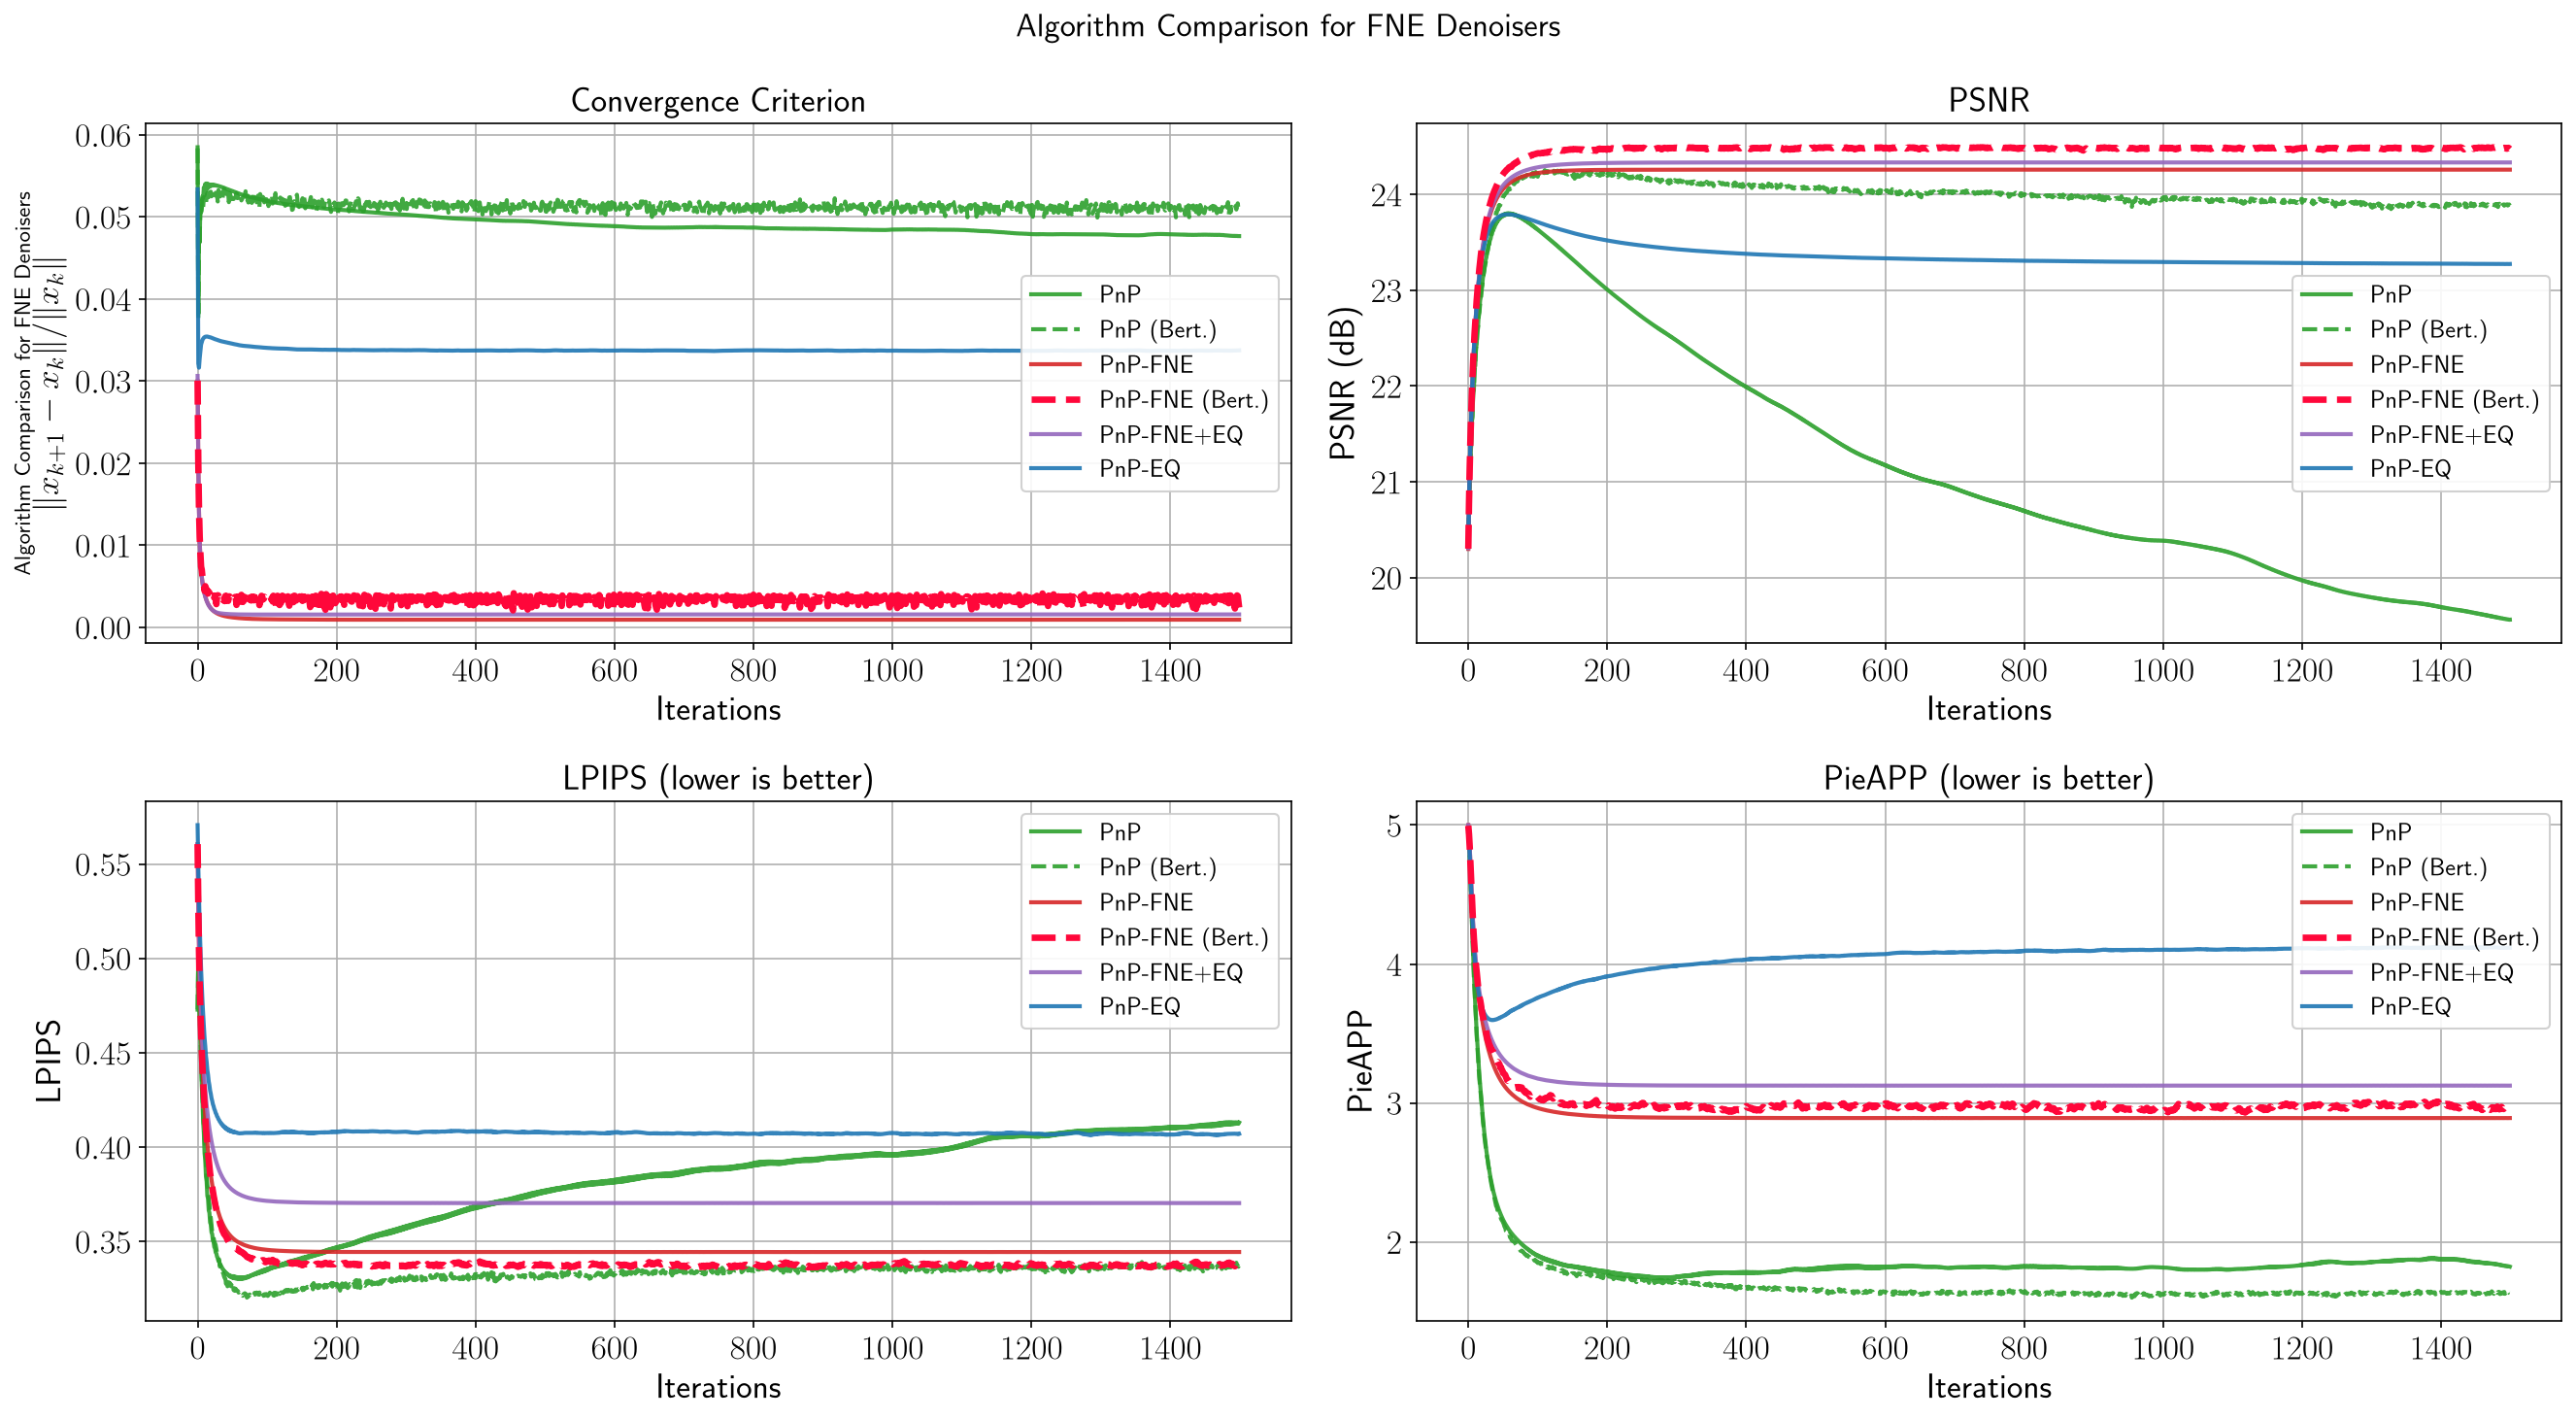
\includegraphics[width=0.9\linewidth]{comparison_curves.png}
%    \caption{Convergence criterion of PnP for the FNE denoiser, compared with the other variants.}
%    \label{fig:convergence-criterion}
%\end{figure*}

%\begin{figure*}[t]
%    \centering
%    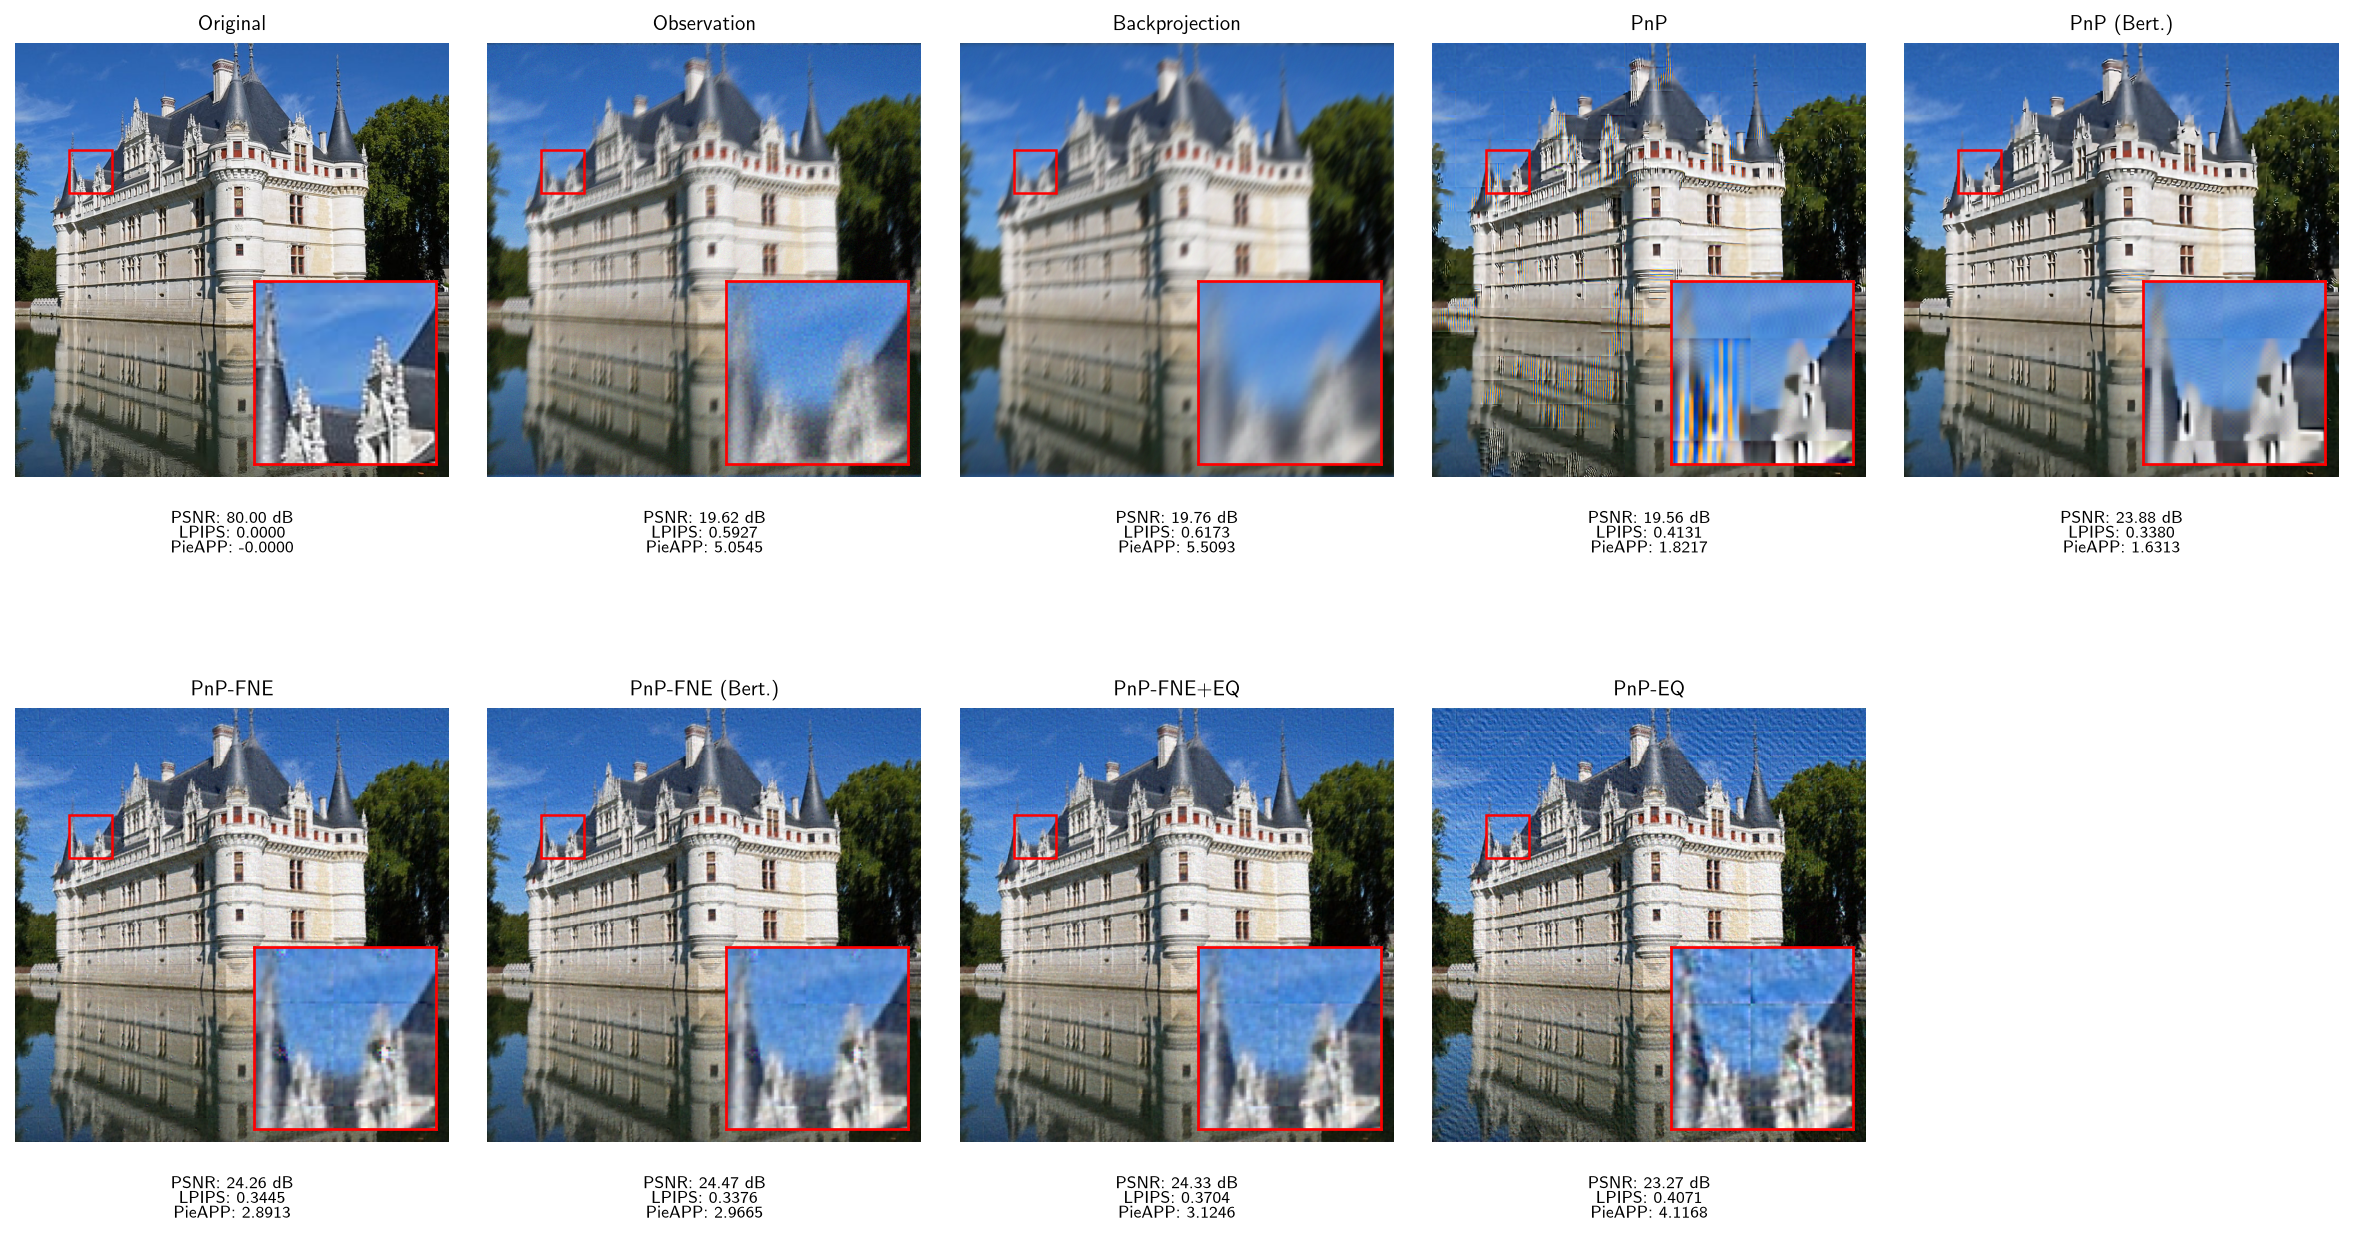
\includegraphics[width=0.9\linewidth]{comparison.png}
%    \caption{PSNR curves across iterations for the different PnP strategies, on the reference experiment.}
%    \label{fig:psnr-reference}
%\end{figure*}

%\begin{figure*}[t]
%    \centering
%    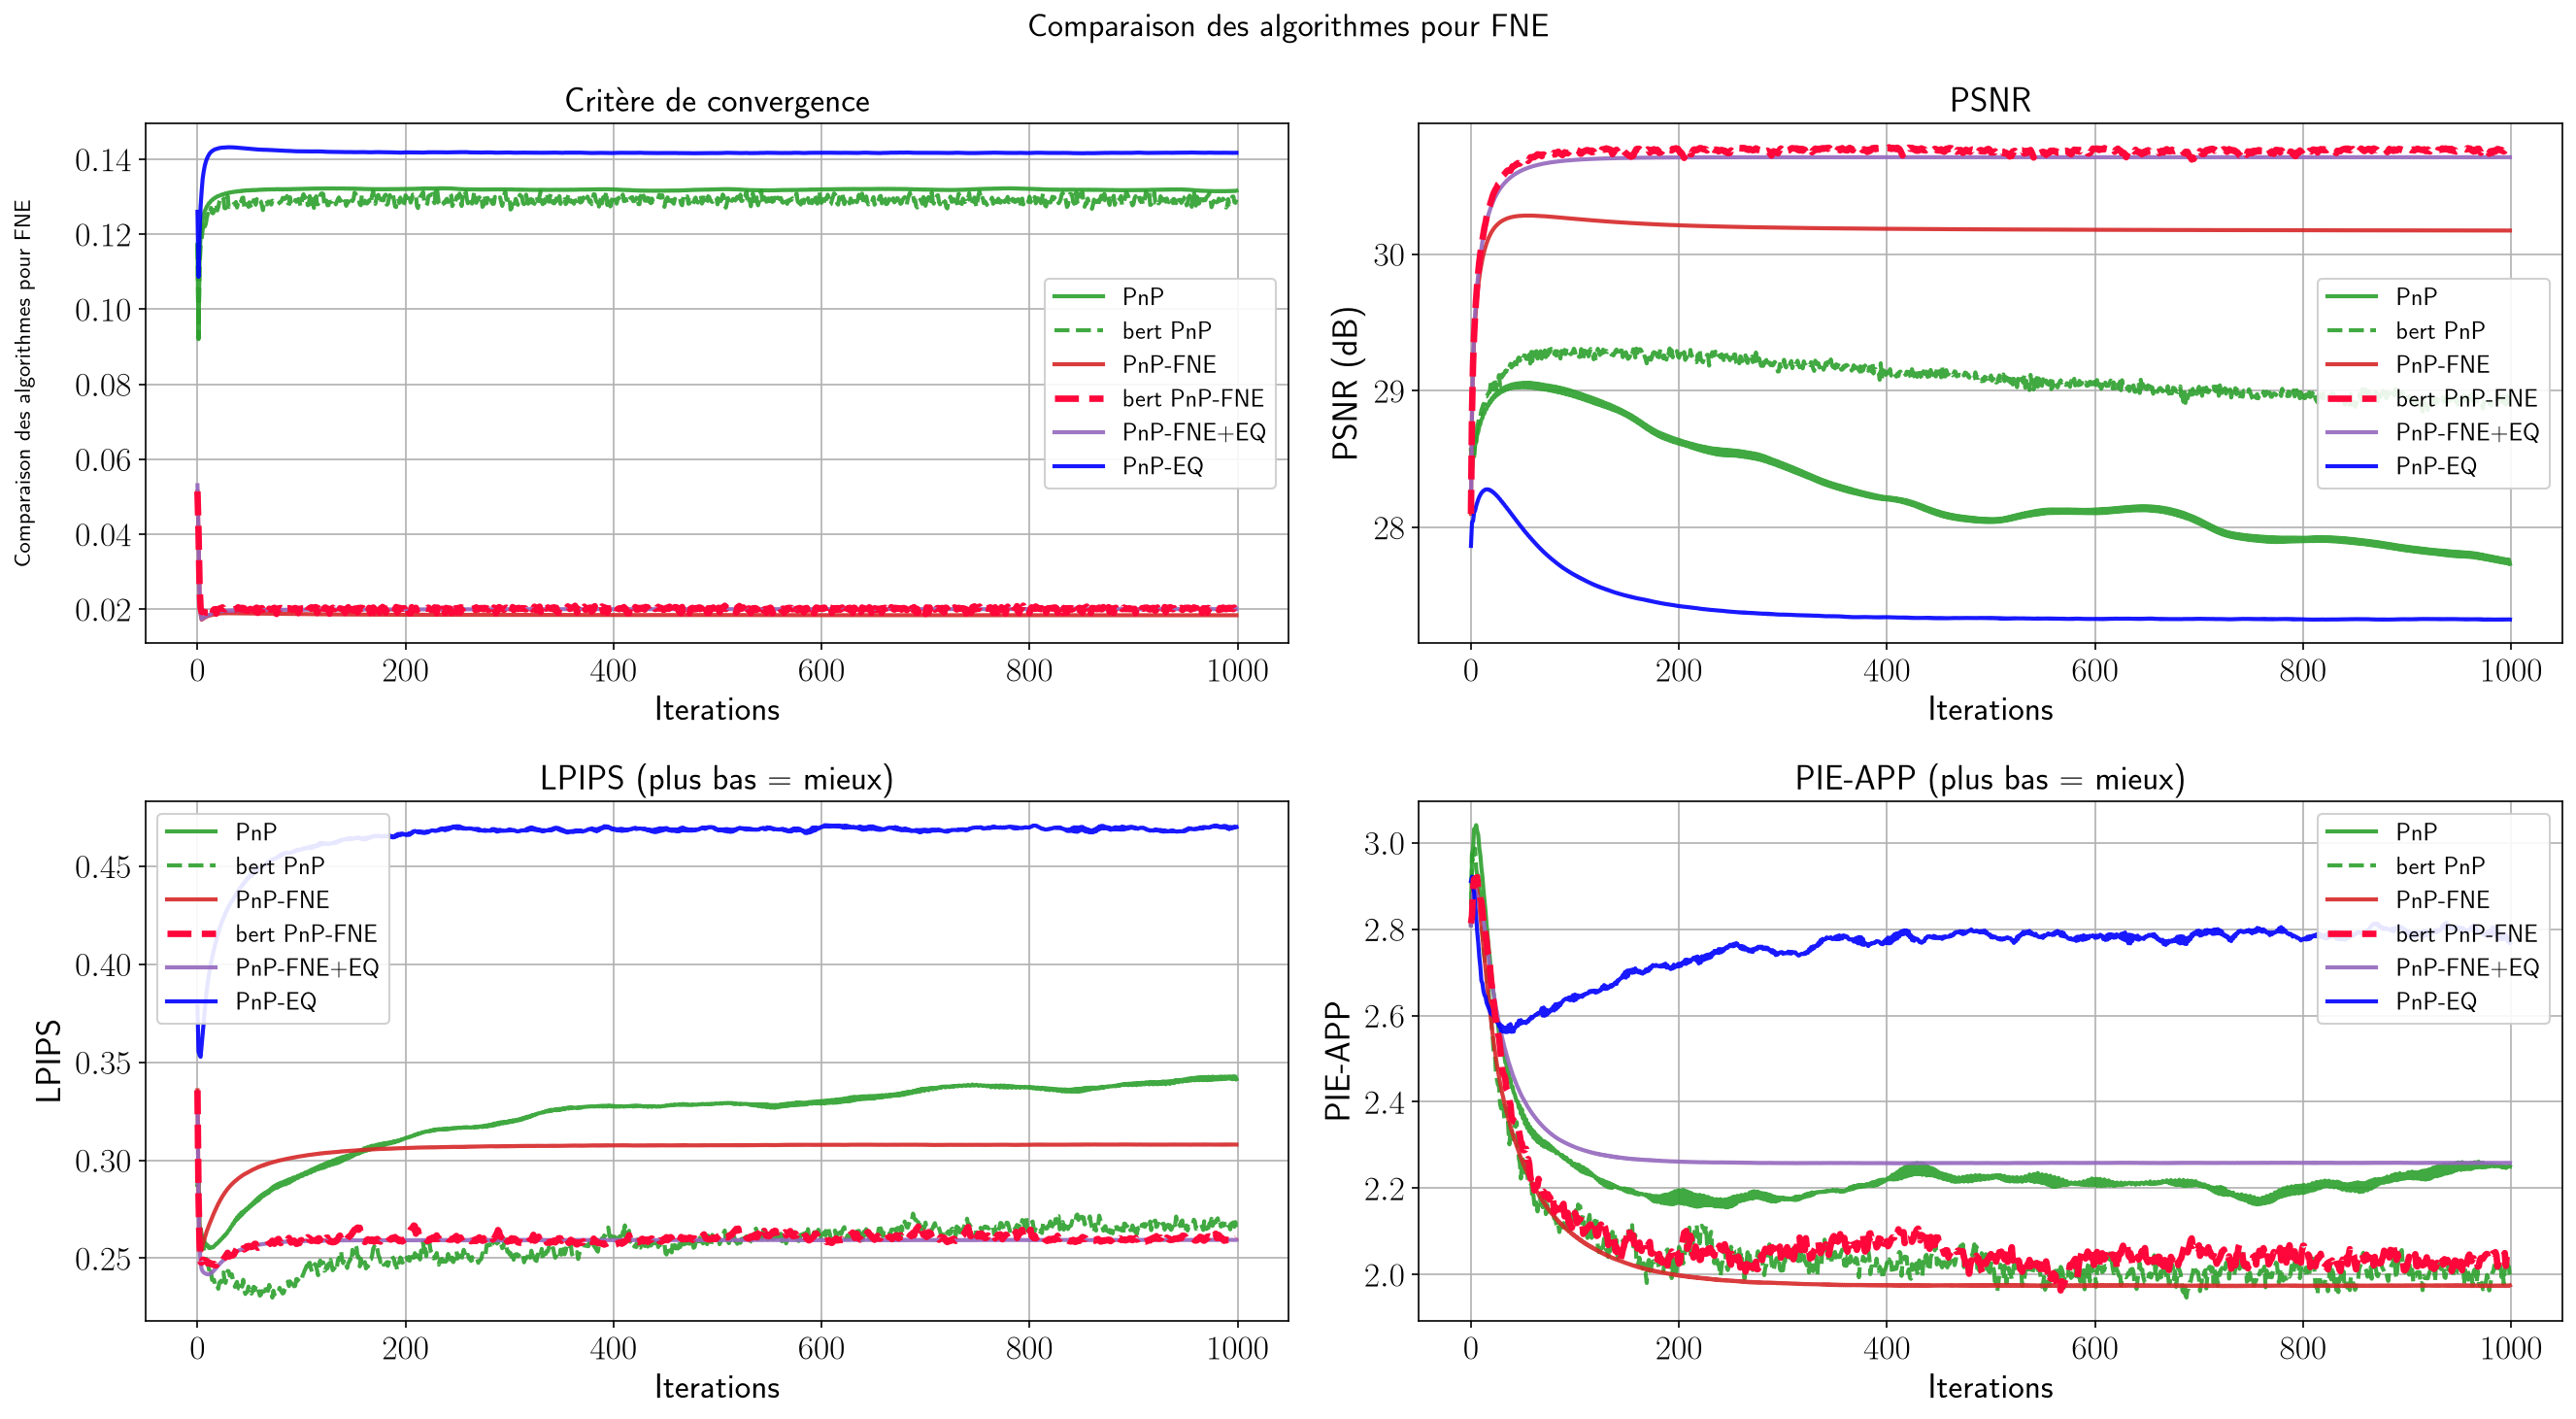
\includegraphics[width=0.9\linewidth]{comparaison_courbes.png}
%    \caption{PSNR curves across iterations, on a second experiment.}
%    \label{fig:psnr-second}
%\end{figure*}

%\begin{figure*}[t]
%    \centering
%    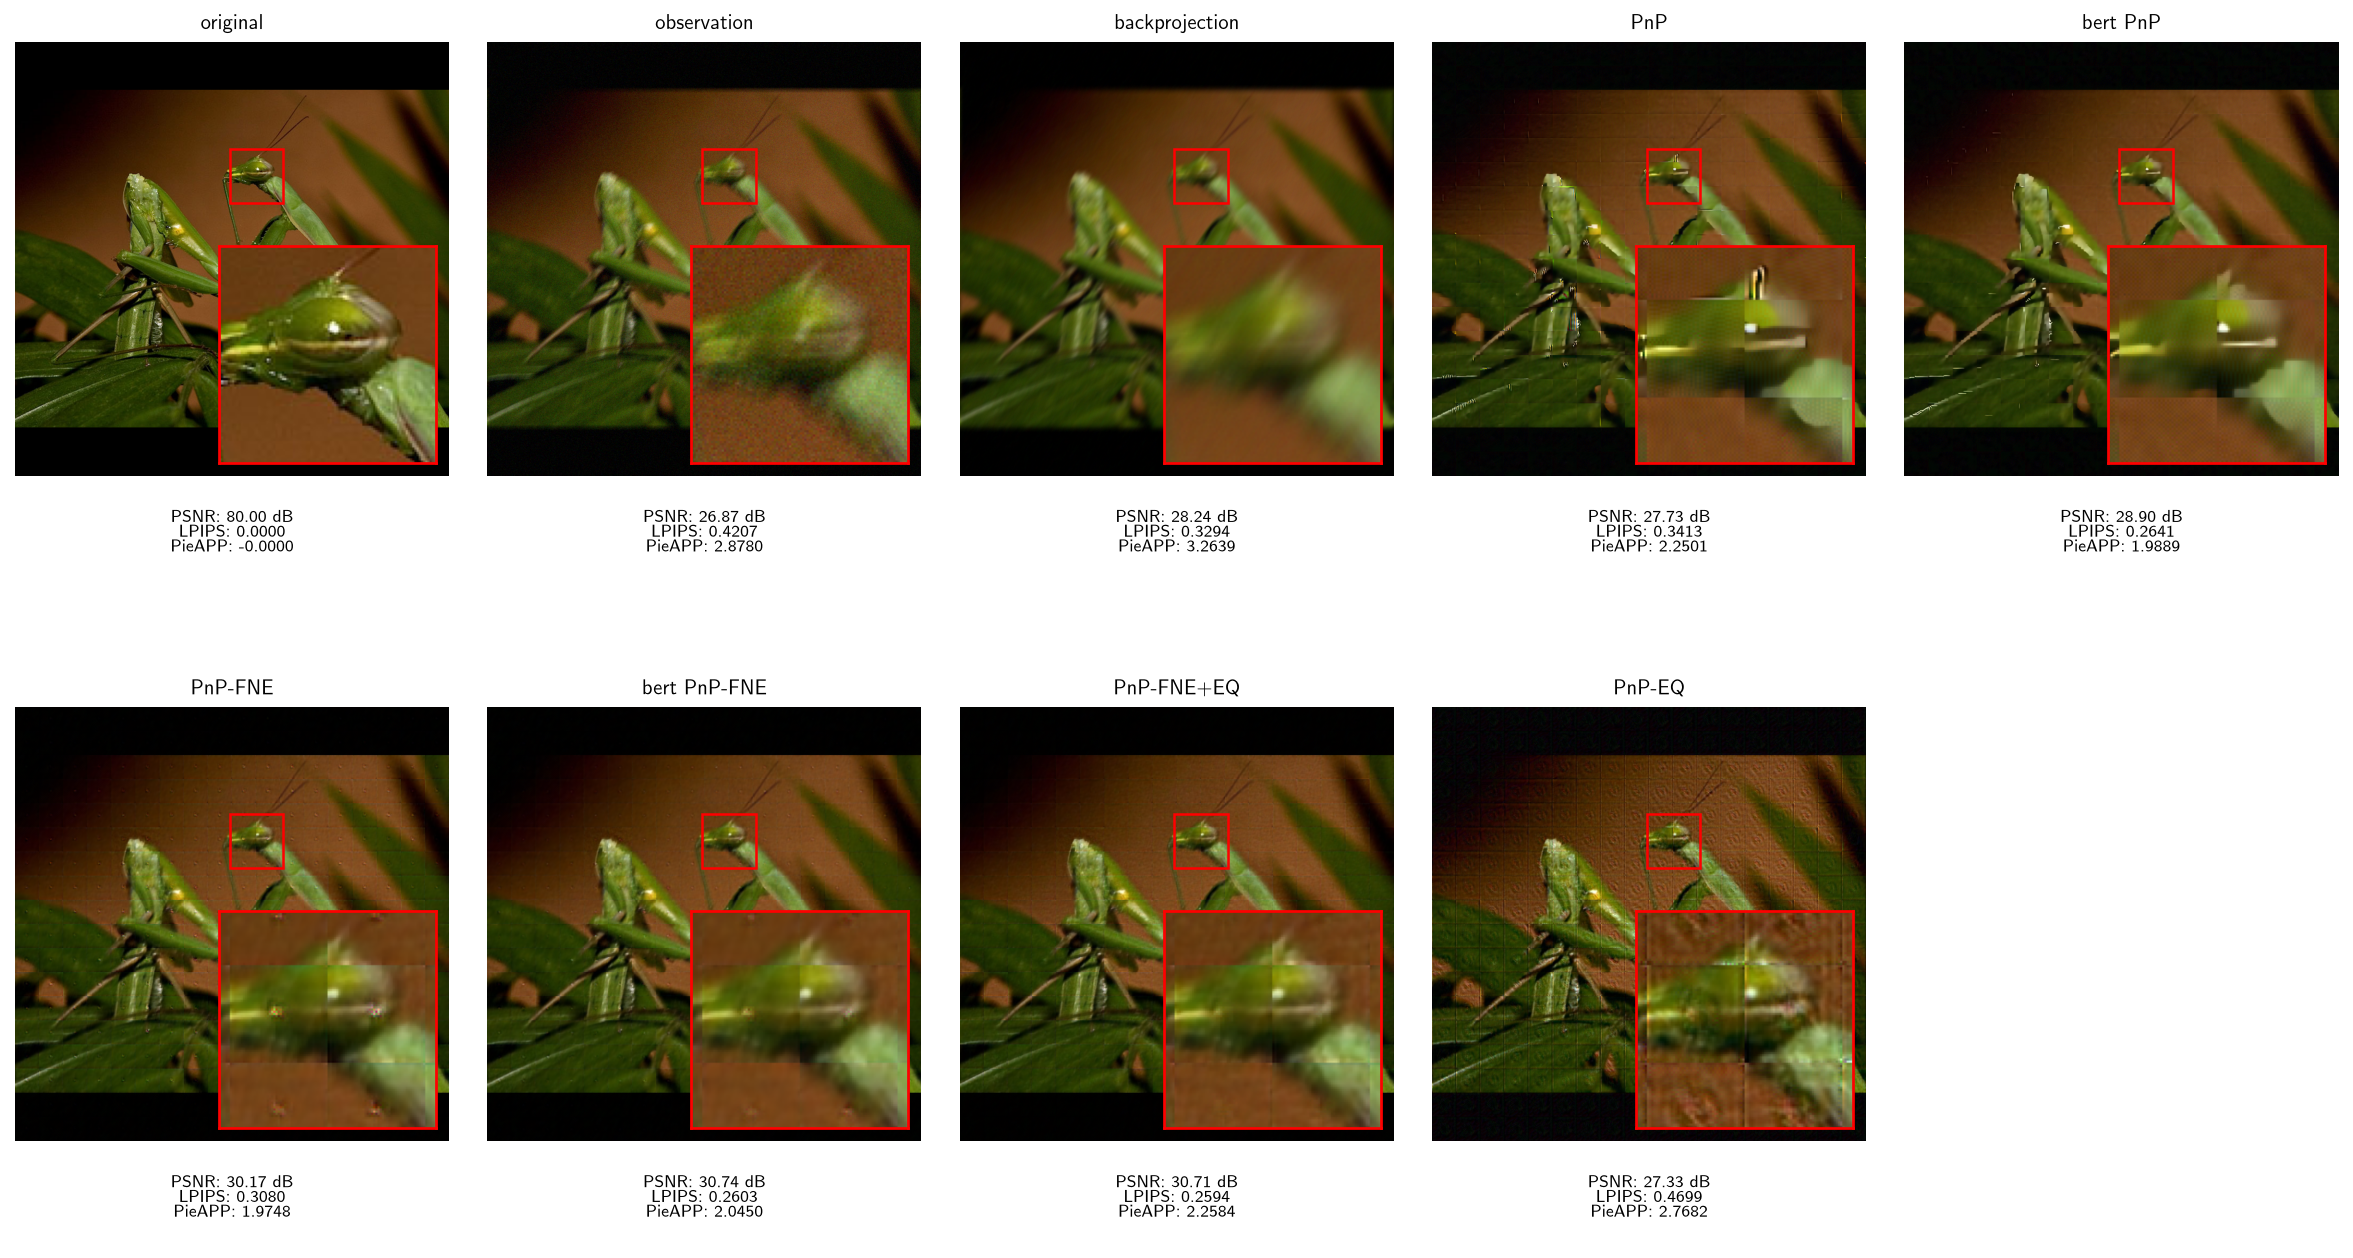
\includegraphics[width=0.9\linewidth]{comparison_mante.png}
%    \caption{Reconstruction obtained by stitching together patches, with and without equivariance at inference time.}
%    \label{fig:patchwork}
%\end{figure*}




\begin{figure}[!h]
\hspace*{-0.5cm}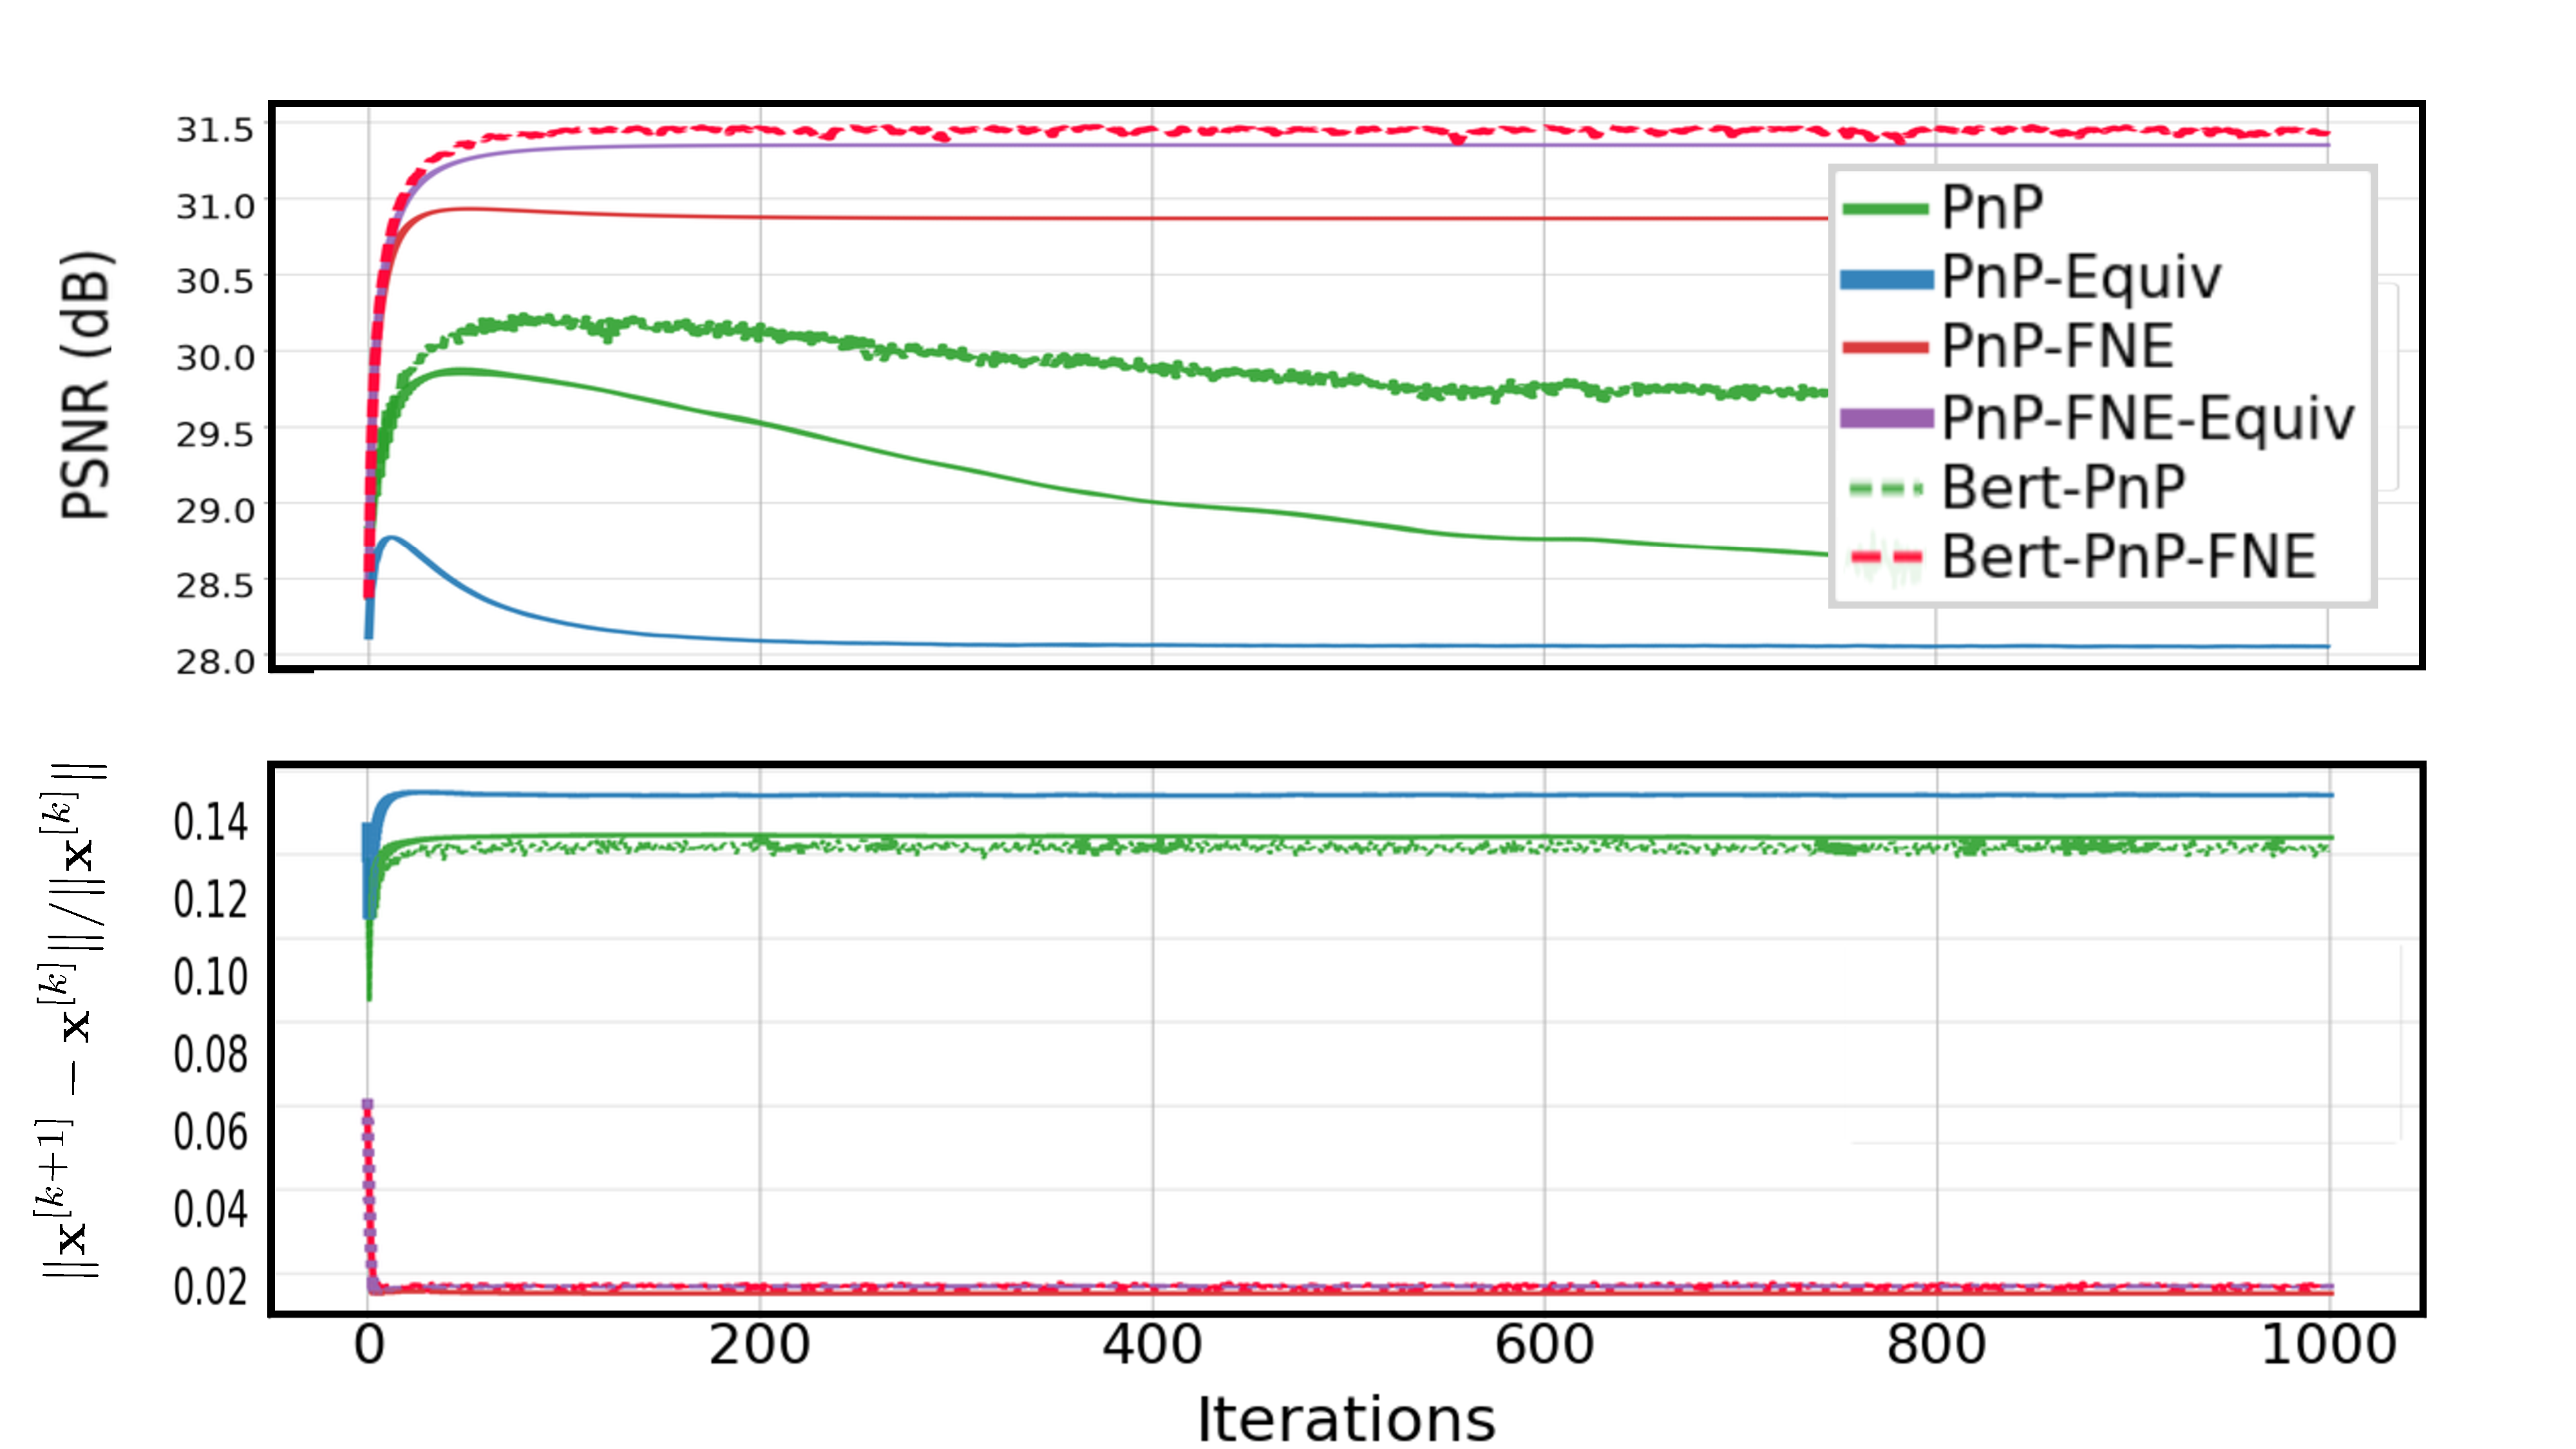
\includegraphics[width = 8.7cm,page=1]{results.pdf} 
\hspace*{-0.5cm}\begin{tabular}{ccc}
     \includegraphics[width=2.3cm, trim=0 1.3cm 0 0, clip]{figures_mante/original.png}&  \includegraphics[width=2.4cm, trim=0 1.3cm 0 0, clip]{figures_mante/observation.png} &
     \includegraphics[width=2.4cm, trim=0 1.3cm 0 0, clip]{figures_mante/backprojection.png}\\  
          Original & Degraded & Backprojection\\
     &PSNR = 26.9dB & PSNR = 28.2dB\\
     \includegraphics[width=2.4cm, trim=0 1.3cm 0 0, clip]{figures_mante/pnp.png} &
     \includegraphics[width=2.4cm, trim=0 1.3cm 0 0, clip]{figures_mante/pnp_equiv.png}&  \includegraphics[width=2.4cm, trim=0 1.3cm 0 0, clip]{figures_mante/pnp_fne.png} \\  
          PnP & PnP-Equiv & PnP-FNE\\
     PSNR = 28.5dB &PSNR = 28.1dB & PSNR = 30.9dB\\
      \includegraphics[width=2.4cm, trim=0 1.3cm 0 0, clip]{figures_mante/pnp_fne_equiv.png}& \includegraphics[width=2.4cm, trim=0 1.3cm 0 0, clip]{figures_mante/bert_pnp.png} &
      \includegraphics[width=2.4cm, trim=0 1.3cm 0 0, clip]{figures_mante/bert_pnp_fne.png} \\ 
           PnP-FNE-Equiv & Bert-PnP & \textbf{Bert-PnP-FNE}\\
     PSNR = 31.4dB &PSNR = 29.7dB & \textbf{PSNR = 31.6dB}\\
\end{tabular}
\caption{{\small{(1st row) PSNR, (2nd row) Residual  (Set of 9 images) Original/degraded and reconstruction results for Image 1.}}\label{fig:res1}}\vspace{-0.6cm}
\end{figure}

\noindent \textbf{Results: Importance of FNE} -- The convergence criteria (PSNR and iterate convergence profiles) are displayed for two images
(Figure~\ref{fig:res1} and Figure~\ref{fig:res2}). Both results are consistent with the theoretical
properties discussed in Section~\ref{sec:bertsekas-reading}. In particular, 
the FNE-regularized variants are the only tested methods for which the residual is observed to converge to zero.
We can also notice that these three strategies {PnP-FNE}, {PnP-FNE-Equiv}, and {Bert-PnP-FNE} achieve the best PSNR performance.

\noindent \textbf{Results: Stochatic Equivariant implementation} --
The PSNR curves, meanwhile, reveal notable differences between the
strategies. 
Overall, equivariance applied at inference in the PnP procedure (i.e., Bert-PnP  or Bert-PnP-FNE)  
brings clearer benefit than equivariance introduced during
training (i.e., PnP-Equiv or PnP-FNE-Equiv). The benefit of equivariance at inference is discussed in more detail
in \cite{Terris2024}. 

\noindent \textbf{Results: FNE and Equivariance} -- From the PSNR plots, both combining equivariance at inference (\textit{i.e.}, Bert-PnP-FNE) or at
training time (\textit{i.e.}, PnP-FNE-Equiv)  lead to better results than the standard FNE
variant (\textit{i.e.}, PnP-FNE). Nonetheless, Bert-PnP-FNE remains slightly better than
PnP-\\%In Figure~\ref{fig:psnr-reference}, the model trained with
%$D_4$ augmentation behaves more stably than PnP with the base
%denoiser. Its performance nonetheless stays below that of FNE,
%especially when FNE is combined with equivariance at inference.





\begin{figure}[!h]
\vspace{-0.9cm}
\hspace*{-0.5cm}\includegraphics[width = 8.7cm,page=2]{results.pdf} 
%\hspace*{-1cm}\includegraphics[width = 9cm, height = 3cm]{figures_chateau/crit.png} \\
\hspace*{-0.5cm}\begin{tabular}{ccc}
     \includegraphics[width=2.3cm, trim=0 1.3cm 0 0, clip]{figures_chateau/original.png}&  
     \includegraphics[width=2.4cm, trim=0 1.3cm 0 0, clip]{figures_chateau/observation.png} &
     \includegraphics[width=2.4cm, trim=0 1.3cm 0 0, clip]{figures_chateau/backprojection.png}\\  
     Original & Degraded & Backprojection\\
     &PSNR = 19.6dB & PSNR = 19.7dB\\
     \includegraphics[width=2.4cm, trim=0 1.3cm 0 0, clip]{figures_chateau/pnp.png} &
     \includegraphics[width=2.4cm, trim=0 1.3cm 0 0, clip]{figures_chateau/pnp_equiv.png}&  \includegraphics[width=2.4cm, trim=0 1.3cm 0 0, clip]{figures_chateau/pnp_fne.png} \\  
     PnP & PnP-Equiv & PnP-FNE\\
     PSNR = 20.4dB &PSNR = 23.3dB & PSNR = 24.3dB\\
      \includegraphics[width=2.4cm, trim=0 1.3cm 0 0, clip]{figures_chateau/pnp_fne_equiv.png}& \includegraphics[width=2.4cm, trim=0 1.3cm 0 0, clip]{figures_chateau/bert_pnp.png} &
      \includegraphics[width=2.4cm, trim=0 1.3cm 0 0, clip]{figures_chateau/bert_pnp_fne.png} \\ 
     PnP-FNE-Equiv & Bert-PnP & \textbf{Bert-PnP-FNE}\\
     PSNR = 24.3dB &PSNR = 24.0dB & \textbf{PSNR = 24.5dB}\\
\end{tabular}
\caption{{\small{(1st row) PSNR, (2nd row) Residual  (Set of 9 images) Original/degraded and reconstruction results for Image 2.}}\label{fig:res2}}
\end{figure}

\noindent FNE-Equiv, while also allowing the use of an FNE denoiser without requiring any retraining.
%Figure~\ref{fig:psnr-second} also shows that, on another experiment,
%the denoiser trained with the equivariance constraint can even
%perform worse than the base PnP. Equivariance applied directly at
%inference, on the other hand, keeps a more consistent effect on
%performance. The FNE constraint again stands out as having the
%biggest impact on reconstruction quality. Combining FNE with
%equivariance at inference therefore gives the best results among the
%methods we studied.

%\begin{figure*}
%\begin{tabular}{cc}
%     \includegraphics[width = 8cm]{figures_chateau/crit.png}&\includegraphics[width = 8cm]{figures_mante/crit.png}\\  \includegraphics[width = 8cm]{figures_chateau/psnr.png}  & \includegraphics[width = 8cm]{figures_mante/psnr.png}\\
%\end{tabular}
%\end{figure*}
%\textbf{This sentence should come earlier.}

\section{Conclusion}\vspace{-0.4cm}

In this work, we showed that equivariant PnP with an FNE denoiser is closely related to Bertsekas incremental proximal-subgradient methods, yielding asymptotic guarantees in the convex case, and we confirmed experimentally in the considered setting, that FNE has the dominant effect of improved equivariance error and reconstruction quality, with data augmentation offering a complementary gain. As future work, extending our convergence proof beyond the convex case remains an open challenge, one that our experimental observations suggest is within reach.
%\textbf{We seem to contradict what is the main claim of the paper. We should move this last paragraph to the conclusion.}
%Finally, equivariance at inference offers an additional benefit for
%image reconstruction. In our experiments (Figure~\ref{fig:patchwork}),
%it seems to help reduce the ``patchwork'' effect seen when an image
%is reconstructed from several patches. This property could be
%especially useful for applications dealing with large images, such
%as medical imaging.

\bibliographystyle{IEEEbib}
\bibliography{refs}

\end{document}
